\documentclass[a4j]{jarticle}
%%  packages
\usepackage{amsmath,amssymb,ascmac}
\usepackage{bm}
\usepackage[dvipdfmx]{graphicx}
\usepackage{listings}
\usepackage[english]{babel}
\lstset{
 	%枠外に行った時の自動改行
 	breaklines = true,
 	%標準の書体
        basicstyle=\ttfamily\footnotesize,
        commentstyle=\footnotesize\bfseries,
        keywordstyle=\footnotesize\bfseries,
 	%枠 "t"は上に線を記載, "T"は上に二重線を記載
	%他オプション:leftline,topline,bottomline,lines,single,shadowbox
 	frame = single,
 	%frameまでの間隔(行番号とプログラムの間)
 	framesep = 5pt,
 	%行番号の位置
 	numbers = left,
	%行番号の間隔
 	stepnumber = 1,
	%タブの大きさ
 	tabsize = 4,
 	%キャプションの場所("tb"ならば上下両方に記載)
 	captionpos = t
}

%% math commands
\let \ds \displaystyle
\newcommand{\idiff}[3]{
  \frac{d^{#1} #2}{d #3^{#1}}
}
\newcommand{\diff}[3]{
  \frac{\mathrm{d}^{#1} #2}{\mathrm{d} #3^{#1}}
}
\newcommand{\pdiff}[3]{
  \frac{\partial^{#1} #2}{\partial #3^{#1}}
}



%% title configuration
\title{ユーザインタフェース レポート}
\author{05-161026 平出一郎}
\date{\today}


%% headings
\pagestyle{headings}
\markright{ユーザインタフェース レポート}




\begin{document}
%%  begin title page
\thispagestyle{empty}
\maketitle
\pagebreak


氏名:平出一郎

所属:情報科学科4年

学籍番号:05-161026

ビデオのURL: https://youtu.be/bf14ep6OASA

実装したクライアントのURL: https://github.com/buko106/VoiceDrive

\section{ユーザインタフェースのデザインと実装}

概要:
\begin{itemize}
\item 声の音量と音の高さで操作する
\end{itemize}

細かい使用方法と動作説明: 

\begin{itemize}
\item マイクに向かって声を出す(母音等は任意)と音量と声の高さを認識する。高い声を出すことで右に曲がり、低い声を出すと左に曲がる。
\item 直進する場合の声の周波数をコマンドラインから与える必要がある。
\item 声を出し続けることで前進する。声を出していないときはブレーキがかかる。
\item スペースキーを押すことでシフトギアを反転する。フィードバックの矢印も反転する。
\item ESCキーでstartコマンドを送信する。
\end{itemize}

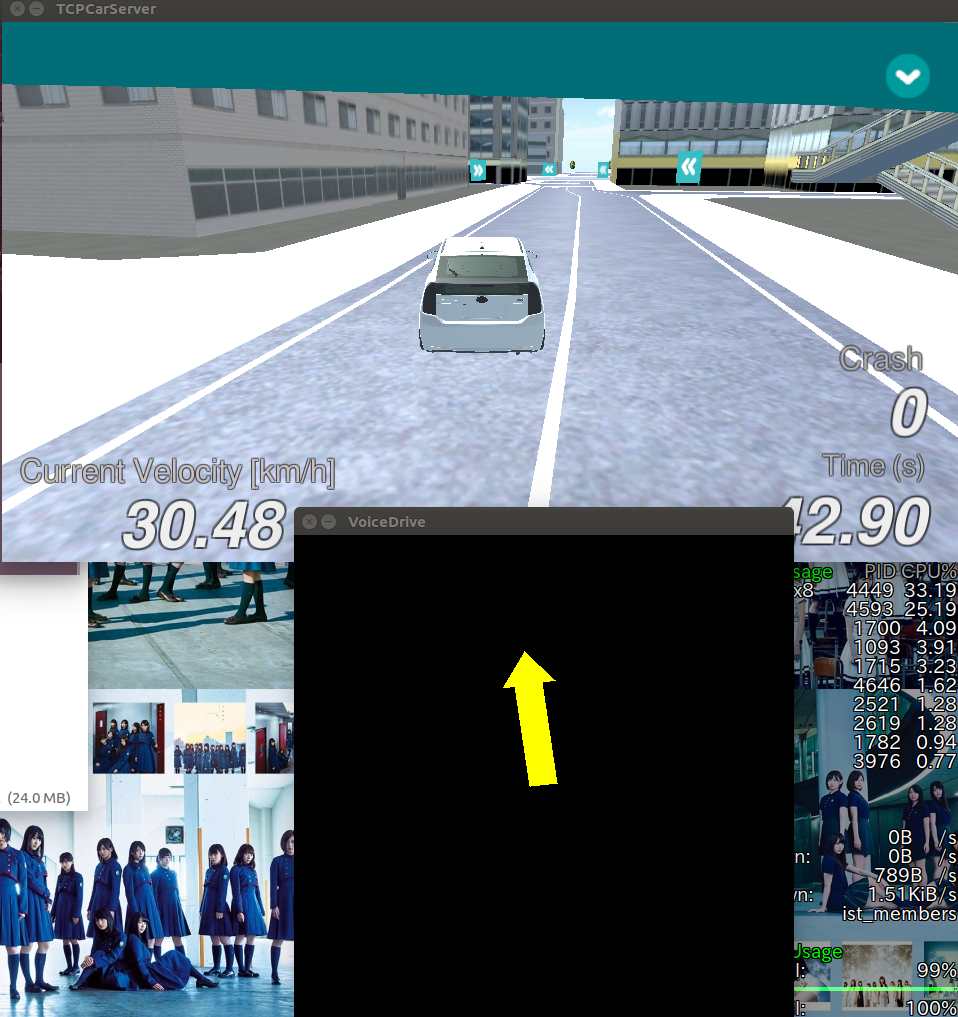
\includegraphics[width=10cm]{captureVoiceDrive.png}

実装にかかった時間:

\begin{itemize}
\item 6時間$\cdots$音声ライブラリの挙動や声に含まれる倍音の影響を調べるなどの試作
\item 4時間$\cdots$チューニングと矢印によるフィードバックの作成
\end{itemize}


\section{ユーザテスト}

被験者のプロファイル:
\begin{itemize}
\item 情報科学科所属の男性(本講義未履修者)2名
\end{itemize}

観察結果:(特に説明なしで触ってみてもらったときの様子)
\begin{itemize}
\item 音の高さによる曲がり具合がわからず、低すぎる声を出す。
\item 声を出し続けないといけないことに気づかず、こま切れに短い声を出す。
\end{itemize}

被験者からのコメント(使いにくかった点や改善案など):
\begin{itemize}
\item 疲れた。腹式呼吸の練習になる。
\item 人目が気になる。
\item 操作は直感的でわかりやすい。
\item 矢印によるフィードバックが良かった。無かったらゴールできないと思う。
\item 息継ぎのために声を切ったときに、切った瞬間の声を感知して左に曲がる。
\item (被験者2)基準音が高かった。
\end{itemize}

実験結果:

\begin{table}[htb]
  \begin{tabular}{crrrrrr}
時間(秒)    & 1回目 & 2回目 & 3回目 & 4回目& 5回目 &平均\\
被験者1 & 72 & 135 & 164 & 72 & 53 & 99\\
被験者2 & 73 & 89 & 47 & 60 & 49 & 64\\
\\
衝突回数(回)    & 1回目 & 2回目 & 3回目 & 4回目& 5回目 & 平均\\
被験者1 & 0 & 6 & 12 & 1 & 0 & 3.8\\
被験者2 & 2 & 7 & 0 & 1 & 0& 2.0\\
  \end{tabular}
\end{table}


\section{まとめ}
全体的な感想、考察など:
\begin{itemize}
\item 想像通りであったが操作は難しい。
\item 暴走を防ぐためにアクセルの最大値に制限を設けたので、早くゴールすることはできなかった。
\item 直進する場合の声の周波数をコマンドラインから与える必要がある(実験では喋り声から私が推定した値を用いた)が、これを基準音をユーザに出してもらいサンプリングする画面を追加したい。
\item ピッチの検出は、倍音の影響を防ぐためにFFTの結果を声の範囲の周波数のみ取り出し周波数の二乗で割った値が最大のものを用いた。ヒューリスティクスではあるが、被験者の男性2名の範囲では問題なく検出ができた。
\item 相対的なピッチの変化を検出するアルゴリズム\footnote{Voice as sound: using non-verbal voice input for interactive control, doi=10.1145/502348.502372}を試したが、ハンドルと上手く対応させる方法を見出だせなかったので採用を見送った。
\end{itemize}

\end{document}


